\newpage
\section{Auswertung}

    \subsection{Kalibirierung des Elektromagneten}
        Die gemessenen Wertepaare aus angelegtem Spulenstrom und erzeugtem Magnetfeld am Ort der Spektrallampe sind in Grafik \ref{fig:Magnetfeld} aufgetragen. Zur Zuordnung einer Magnetfeldstärke B zu einem 
        angelegten Spulenstrom I, wird eine Funktion dritter Ordnung an die Werte angepasst. So ergibt sich die Funktion

        \begin{equation}
            B(I) = aI^3 + bI^2 + cI + d
            \label{eqn:kalibration}
        \end{equation}
        
        mit den Parametern 

        \begin{equation*}
          a =\SI{-0.0005626}{\tesla \per \ampere^3} \qquad b =\SI{0.00026665}{\tesla \per \ampere^2} \qquad c =\SI{0.10692288}{\tesla \per \ampere}   \qquad   d =\SI{-0.00662435}{\tesla },
        \end{equation*}
            
        die die Magnetfeldstärke in Tesla angibt.
        \FloatBarrier

        \begin{figure}[h]
          \centering
          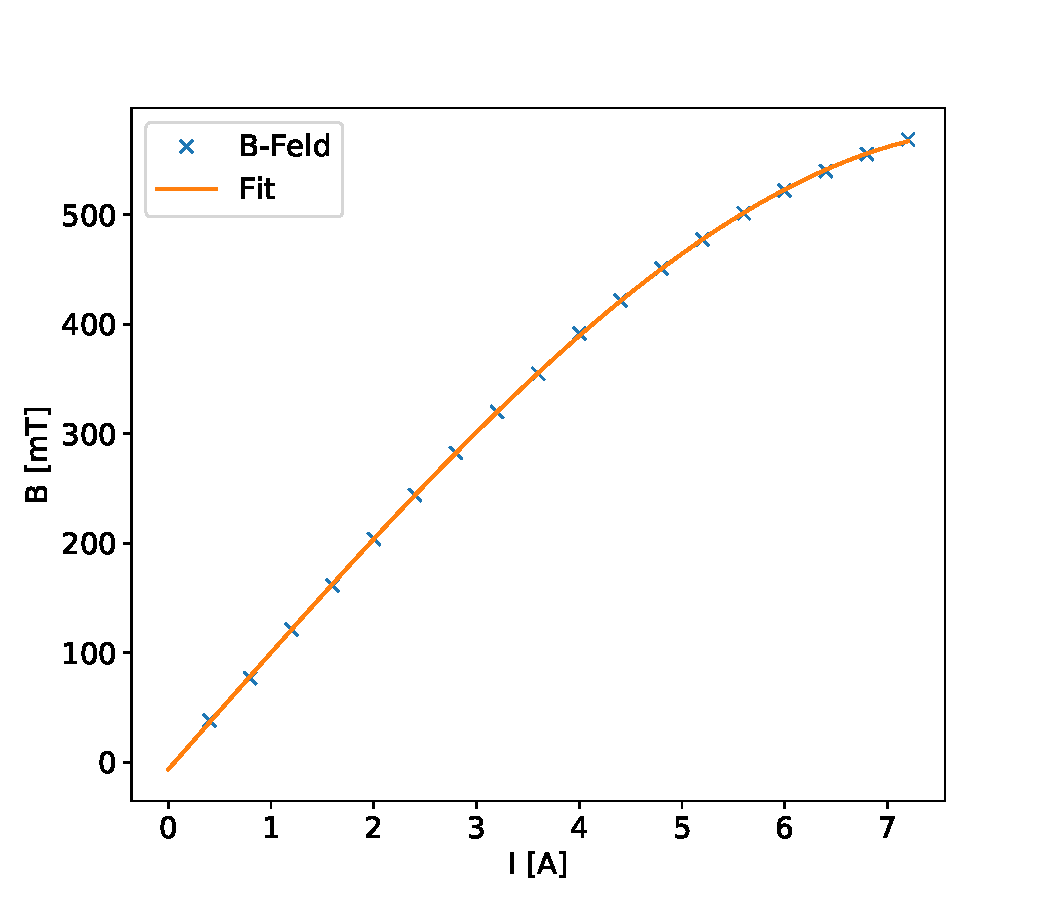
\includegraphics[width = 0.6\textwidth]{magnetfeld.pdf}
          \caption{Die gemessenen Magnetfeldstärken B sind gegen die angelegten Stromstärken I aufgetragen. Zur Beschreibung des Zusammenhangs wird ein Polynom dritter Ordnung an die Messwerte angepasst.}
          \label{fig:Magnetfeld}
        \end{figure}
    
        \FloatBarrier

    \newpage
    \subsection{Bestimmung der Wellenlängenaufspaltung}
        In der folgenden Auswertung wird angenommen, dass die Abstände im Interferenzmuster mit einem Fehler von $\pm 1$ Pixel abgelesen werden. Die daraus resultierenden Fehler werden über die Gauß´sche
        Fehlerfortpflanzung berechnet. Dabei berechnet sich der Fehler $\Delta f$ einer Größe, die aus fehlerbehafteten Größen berechnet wird über folgende Formel
        
        \begin{equation*}
          \Delta f = \sqrt{\sum_{i=1}^N (\frac{df}{dy_i}\cdot \Delta y_i)^2},
        \end{equation*}

        in der $N$ für die Anzahl der einfließenden, fehlerbehafteten Größen und $y_i$ bzw. $\Delta y_i$ für die fehlerbehaftete Größe und deren Fehler steht.

        \subsubsection*{Untersuchung des 643,8\,nm-Übergangs}
            Zunächst wird die Verschiebung der Maxima im Interferenzmuster für den roten Übergang der Wellenlänge \SI{643.8}{\nano\metre} untersucht. Für eine Einstellung des Polarisators auf 90° wird wie aus
            der Geometrie des Aufbaus zu erwarten keine Aufspaltung der Interferenzmaxima beobachtet.

            \FloatBarrier

            \begin{figure}[h]
              \centering
              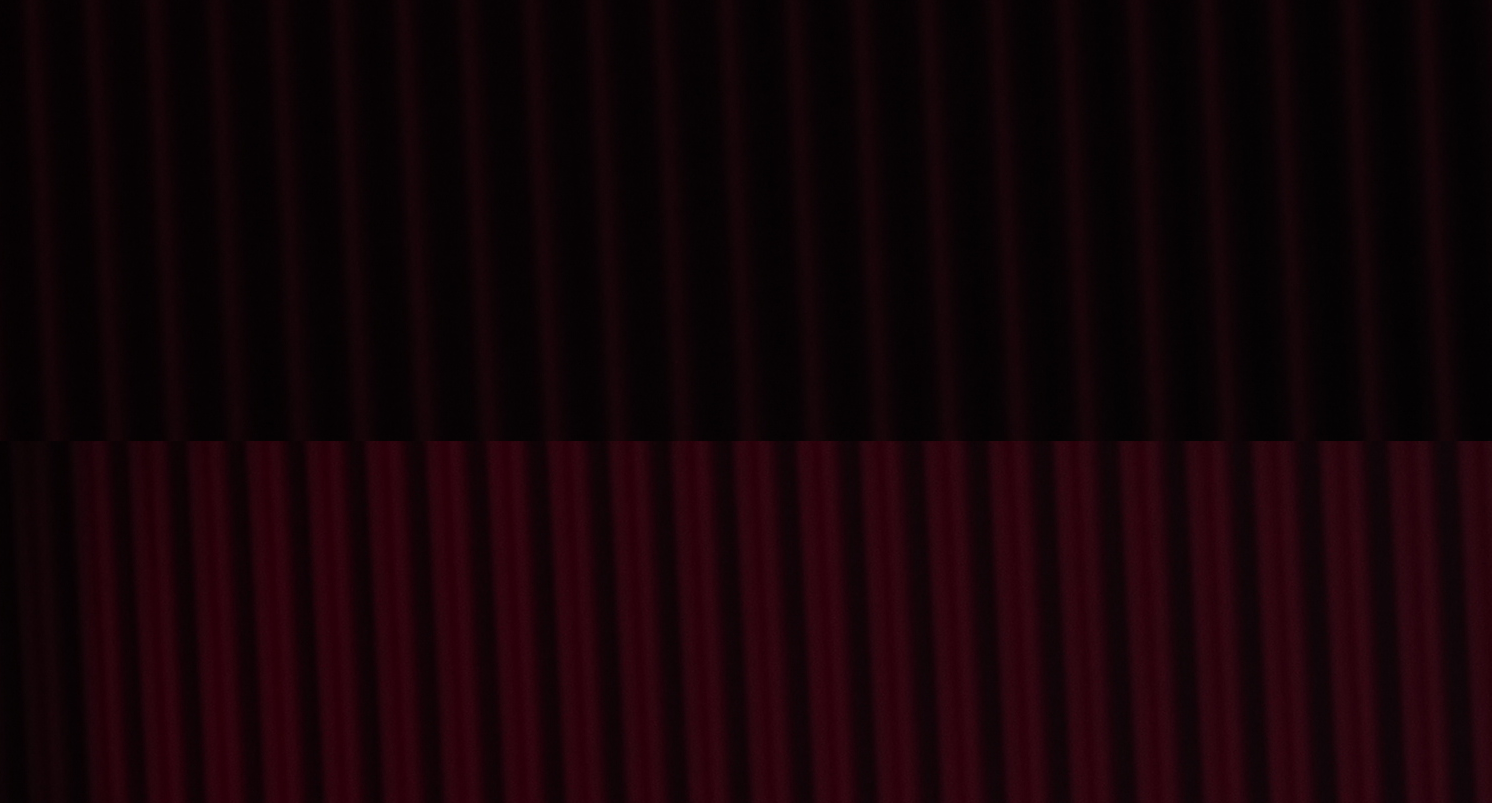
\includegraphics[width = 0.6\textwidth]{pictures/rot_sigma.png}
              \caption{Das per Digitalkamera aufgenommene Interferenzmuster bei ausgeschaltetem Magnetfeld (oben) und das verschobene Interferenzmuster bei einer Magnetfeldstärke von \SI{465}{\milli\tesla} (unten) für den $\sigma$-polarisierten Anteil des 643,8\,nm-Übergangs.}
              \label{fig:rot_sigma}
            \end{figure}
        
            \FloatBarrier

            Durch Einstellen des Polarisators auf 90° wird der $\sigma$-polarisierte Anteil des Lichts untersucht. Hier stellt sich wie Abbildung \ref{fig:rot_sigma} zu sehen bei einem angelegten Magnetfeld von 
            \SI{465}{\milli\tesla}, das über Formel \ref{eqn:kalibration} für einen Spulenstrom von \SI{5}{\ampere} bestimmt wurde, eine Verschiebung der Interferenzmaxima ein. Aus dem Interferenzmuster bei 
            ausgeschaltetem Magnetfeld wird der Abstand zwischen den Maxima ohne Zeeman-Aufspaltung $\Delta s$
            für 13 Maxima ermittelt. Analog wird die Aufspaltung der Maxima bei eingeschaltetem Magnetfeld $\delta s$ aus dem aufgenommenen Interferenzmuster abgelesen. Diese Werte sowie die daraus über Formel
            \ref{eqn:delta_lambda} berechnete Verschiebung der Wellenlänge $\delta\lambda$ sind in Tabelle \ref{tab:rot_sigma} aufgelistet. Aus diesen wird die mittlere Wellenlängeverschiebung berechnet, die sich 
            zu

            \begin{equation*}
                \overline{\delta \lambda_{\text{rot}, \sigma}} = \left(8,92 \pm 0,12\right)\si{\pico\metre}.
            \end{equation*}

            ergibt. Mit dieser wird der Landè-Faktor g berechnet, indem die Energieaufspaltung $\Delta E$ \ref{eqn:E} nach diesem umgestellt wird und diese Energieänderung aufgrund der 
            Zeeman-Aufspaltung über 

            \begin{equation*}
                \Delta E = \frac{\delta E}{\delta \lambda} E(\lambda) \qquad \text{mit} \qquad E(\lambda) = \frac{\text{hc}}{\lambda}
            \end{equation*}

            mit der Wellenlängenverschiebung verknüpft wird. Der Landé-Faktor ergibt sich so über
            
            \begin{equation}
              g = \frac{\delta\lambda\text{hc}}{\mu_{\text{B}}B\lambda^2}
              \label{eqn:Lande}
            \end{equation}
            
            zu

            \begin{equation*}
                g_{\text{rot}, \sigma} = 0,993 \pm 0,013 .
            \end{equation*}


            \begin{table}[h]
                \centering
                \caption{Die abgelesenen Abstände der Interferenzmaxima $\Delta s_{\text{rot}, \sigma}$ bei ausgeschaltetem Magnetfeld, die Aufspaltung der Interferenzmaxima $\delta s_{\text{rot}, \sigma}$ sowie die berechnete Wellenlängeverschiebung $\delta \lambda_{\text{rot}, \sigma}$}
                \label{tab:rot_sigma}
              
                \begin{tabular}{c c c}
                  \toprule
                  {$\Delta s_{\text{rot}, \sigma}$ [Pixel]} & {$\delta s_{\text{rot}, \sigma}$ [Pixel]} & {$\delta \lambda_{\text{rot}, \sigma}$ [\si{\pico\metre}]} \\ 
                  \midrule
                   61 $\pm$ 1  &   23 $\pm$ 1   &   9,22 $\pm$ 0,43   \\
                   61 $\pm$ 1  &   21 $\pm$ 1   &   8,42 $\pm$ 0,43   \\
                   62 $\pm$ 1  &   23 $\pm$ 1   &   9,08 $\pm$ 0,43   \\
                   60 $\pm$ 1  &   22 $\pm$ 1   &   8,97 $\pm$ 0,44   \\
                   61 $\pm$ 1  &   23 $\pm$ 1   &   9,23 $\pm$ 0,43   \\
                   61 $\pm$ 1  &   23 $\pm$ 1   &   9,23 $\pm$ 0,43   \\
                   61 $\pm$ 1  &   23 $\pm$ 1   &   9,08 $\pm$ 0,43   \\
                   62 $\pm$ 1  &   23 $\pm$ 1   &   9,47 $\pm$ 0,43   \\
                   62 $\pm$ 1  &   24 $\pm$ 1   &   8,54 $\pm$ 0,42   \\
                   63 $\pm$ 1  &   22 $\pm$ 1   &   8,41 $\pm$ 0,41   \\
                   64 $\pm$ 1  &   22 $\pm$ 1   &   8,90 $\pm$ 0,40   \\
                   65 $\pm$ 1  &   24 $\pm$ 1   &   9,17 $\pm$ 0,41   \\
                   61 $\pm$ 1  &   24 $\pm$ 1   &   8,28 $\pm$ 0,40   \\

                  \bottomrule
                \end{tabular}
              \end{table}
              \FloatBarrier

        \newpage
        \subsubsection*{Untersuchung des 480,0\,nm-Übergangs}
            Anschließend wird die Verschiebung der Maxima im Interferenzmuster für den blauen Übergang der Wellenlänge \SI{480}{\nano\metre} untersucht. Hier wird zunächst der Übergang mit $\pi$-polarisertem
            Licht untersucht. Dazu wurden die Daten eines externen Versuches genutzt, bei dem das angelegte Magnetfeld \SI{1009}{\milli\tesla} betrug.
            Analog zur Auswertung des roten Übergangs 
            werden die benötigten Abstände aus den in Abbildung \ref{fig:blau_pi} zu sehenden Interferenzmustern abgelesen. Die Ergebnisse sind in 
            Tabelle \ref{tab:blau_pi} aufgelistet und werden genutzt, um die mittlere Wellenlängeverschiebung und den Landé-Faktor analog zu dem Vorgehen beim roten Übergang zu berechnen. So ergeben sich die
            Wellenlängenverschiebung zu

            \begin{equation*}
                \overline{\delta \lambda_{\text{blau}, \pi}} = \left(6,18 \pm 0,10\right)\si{\pico\metre}
            \end{equation*}

            und der Landé-Faktor zu

            \begin{equation*}
              g_{\text{blau}, \pi} = 0,663 \pm 0,004 .
            \end{equation*}

            \FloatBarrier

            \begin{figure}[h]
              \centering
              
\includegraphics[width = 0.6\textwidth]{pictures/blau_pi.png}
              \caption{Das per Digitalkamera aufgenommene Interferenzmuster bei ausgeschaltetem Magnetfeld (oben) und das verschobene Interferenzmuster bei einer Magnetfeldstärke von \SI{1009}{\milli\tesla} (unten) für den $\pi$-polarisierten Anteil des 480\,nm-Übergangs.}
              \label{fig:blau_pi}
            \end{figure}
        
            \FloatBarrier

              \begin{table}[h]
                \centering
                \caption{Die abgelesenen Abstände der Interferenzmaxima $\Delta s_{\text{blau}, \pi}$ bei ausgeschaltetem Magnetfeld, die Aufspaltung der Interferenzmaxima $\delta s_{\text{blau}, \pi}$ sowie die berechnete Wellenlängeverschiebung $\delta \lambda_{\text{blau}, \pi}$}
                \label{tab:blau_pi} 
              
                \begin{tabular}{c c c}
                  \toprule
                  {$\Delta s_{\text{blau}, \pi}$ [Pixel]} & {$\delta s_{\text{blau}, \pi}$ [Pixel]} & {$\delta \lambda_{\text{blau}, \pi}$ [\si{\pico\metre}]} \\ 
                  \midrule
                   123 $\pm$ 1  &   63 $\pm$ 1   &   6,90 $\pm$ 0,13   \\
                   125 $\pm$ 1  &   59 $\pm$ 1   &   6,36 $\pm$ 0,12   \\
                   113 $\pm$ 1  &   61 $\pm$ 1   &   7,27 $\pm$ 0,14   \\
                   114 $\pm$ 1  &   59 $\pm$ 1   &   6,97 $\pm$ 0,14   \\
                   108 $\pm$ 1  &   57 $\pm$ 1   &   7,11 $\pm$ 0,15   \\
                   103 $\pm$ 1  &   53 $\pm$ 1   &   6,93 $\pm$ 0,15   \\
                   101 $\pm$ 1  &   55 $\pm$ 1   &   7,34 $\pm$ 0,16   \\
                   100 $\pm$ 1  &   53 $\pm$ 1   &   7,14 $\pm$ 0,16   \\
                   92  $\pm$ 1  &   45 $\pm$ 1   &   6,59 $\pm$ 0,17   \\
                   92  $\pm$ 1  &   49 $\pm$ 1   &   7,18 $\pm$ 0,17   \\
                   91  $\pm$ 1  &   55 $\pm$ 1   &   8,14 $\pm$ 0,18   \\
                   92  $\pm$ 1  &   53 $\pm$ 1   &   7,76 $\pm$ 0,17   \\
                   88  $\pm$ 1  &   51 $\pm$ 1   &   7,81 $\pm$ 0,18   \\

                  \bottomrule
                \end{tabular}
              \end{table}
              \FloatBarrier


              Zuletzt wird der Übergang mit $\sigma$-polarisiertem Licht untersucht. Hier wird die Magnetfeldstärke über die Kalibirierung für einen Spulenstrom von \SI{2.6}{\ampere} 
              zu \SI{263}{\milli\tesla} bestimmt. Per analogem Vorgehen zu den vorherigen Übergängen werden die in Tabelle \ref{tab:blau_sigma} aufgelisteten Werte wieder aus
              den in Abbildung \ref{fig:blau_sigma} zu sehenden Interferenzbildern abgelesen. Die mittlere Wellenlängenverschiebung ergibt sich zu

            \begin{equation*}
              \overline{\delta \lambda_{\text{blau}, \sigma}} = \left(6,18 \pm 0,10\right)\si{\pico\metre}
            \end{equation*}

            und der Landé-Faktor wird daraus zu

            \begin{equation*}
              g_{\text{blau}, \sigma} = 2,180 \pm 0,040 
            \end{equation*}

            bestimmt.



              \FloatBarrier

              \begin{figure}[h]
                \centering
                
\includegraphics[width = 0.6\textwidth]{pictures/blau_sigma.jpg}
                \caption{Das per Digitalkamera aufgenommene Interferenzmuster bei ausgeschaltetem Magnetfeld (oben) und das verschobene Interferenzmuster bei einer Magnetfeldstärke von \SI{263}{\milli\tesla} (unten) für den $\sigma$-polarisierten Anteil des 480\,nm-Übergangs.}
                \label{fig:blau_sigma}
              \end{figure}
          
              \FloatBarrier

              \begin{table}[h]
                \centering
                \caption{Die abgelesenen Abstände der Interferenzmaxima $\Delta s_{\text{blau}, \sigma}$ bei ausgeschaltetem Magnetfeld, die Aufspaltung der Interferenzmaxima $\delta s_{\text{blau}, \sigma}$ sowie die berechnete Wellenlängeverschiebung $\delta \lambda_{\text{blau}, \sigma}$}
                \label{tab:blau_sigma}
              
                \begin{tabular}{c c c}
                  \toprule
                  {$\Delta s_{\text{blau}, \sigma}$ [Pixel]} & {$\delta s_{\text{blau}, \sigma}$ [Pixel]} & {$\delta \lambda_{\text{blau}, \sigma}$ [\si{\pico\metre}]} \\ 
                  \midrule
                   40 $\pm$ 1  &   19 $\pm$ 1   &   6,40 $\pm$ 0,38   \\
                   41 $\pm$ 1  &   20 $\pm$ 1   &   6,57 $\pm$ 0,37   \\
                   42 $\pm$ 1  &   18 $\pm$ 1   &   5,78 $\pm$ 0,35   \\
                   40 $\pm$ 1  &   19 $\pm$ 1   &   6,40 $\pm$ 0,38   \\
                   40 $\pm$ 1  &   20 $\pm$ 1   &   6,74 $\pm$ 0,38   \\
                   41 $\pm$ 1  &   20 $\pm$ 1   &   6,57 $\pm$ 0,37   \\
                   40 $\pm$ 1  &   18 $\pm$ 1   &   6,06 $\pm$ 0,37   \\
                   40 $\pm$ 1  &   18 $\pm$ 1   &   6,06 $\pm$ 0,37   \\
                   40 $\pm$ 1  &   17 $\pm$ 1   &   5,73 $\pm$ 0,37   \\
                   42 $\pm$ 1  &   18 $\pm$ 1   &   5,78 $\pm$ 0,36   \\
                   41 $\pm$ 1  &   18 $\pm$ 1   &   5,92 $\pm$ 0,37   \\
                   40 $\pm$ 1  &   18 $\pm$ 1   &   6,06 $\pm$ 0,38   \\
                   39 $\pm$ 1  &   18 $\pm$ 1   &   6,22 $\pm$ 0,39   \\

                  \bottomrule
                \end{tabular}
              \end{table}
              \FloatBarrier
            
            